%!TEX root = ../template.tex
%%%%%%%%%%%%%%%%%%%%%%%%%%%%%%%%%%%%%%%%%%%%%%%%%%%%%%%%%%%%%%%%%%%%
%% chapter4.tex
%% NOVA thesis document file
%%
%% Chapter with lots of dummy text
%%%%%%%%%%%%%%%%%%%%%%%%%%%%%%%%%%%%%%%%%%%%%%%%%%%%%%%%%%%%%%%%%%%%

\typeout{NT FILE chapter4.tex}%

\chapter{Preliminary Results}
\label{cha:Preliminary_Results}

This chapter presents the goal pipeline, the initial tool modifications already implemented and a set of manually derived examples that 
illustrate how \ocaml + \gospel code can be correctly translated into 
semantically equivalent \cml representations. These examples serve as a reference for the expected behaviour and structure of verified 
translations. The goal is to demonstrate the existing tools for translation into \cml and identifying what the corresponding \cml code 
should look like in order to compile successfully and preserve the intended behaviour.

\section{Goal Pipeline}

After analysing the verification pipeline in figure \ref{fig:Cameleer_pipeline} it is possible to observe that some parts have already been 
implemented or require only minor adjustments to meet their objectives. By modifying the extraction process in \whythree to check if the 
proof has been discharged we can provide better correctness guarantees because the generated \cml code will comply to the specification. 
Due to differences in syntax and features that have no direct equivalents in \cml, we must also include some kind of error message for 
failures in extraction, for instance the lack of support for \inlinecode{while} and \inlinecode{for} loops.

The main goal of this work is to expand the currently available pipeline of translating code from \ocaml with \gospel specifications 
into \whyml, where it can be verified using the various automated provers available in \whythree. We want to achieve 
a more robust extraction mechanism with the ideas as previously discussed. Moreover, we ought to provide a new tool that 
translates a subset of compilable \cml code with \gospel annotations into \ocaml with \gospel equivalents that can later
prove their correctness in \cameleer. Creating this translation tool for a certified compiler like \cml is particularly valuable for 
research and comparative analysis. The figure below represents the goal pipeline:

\begin{figure}[H]
    \centering
    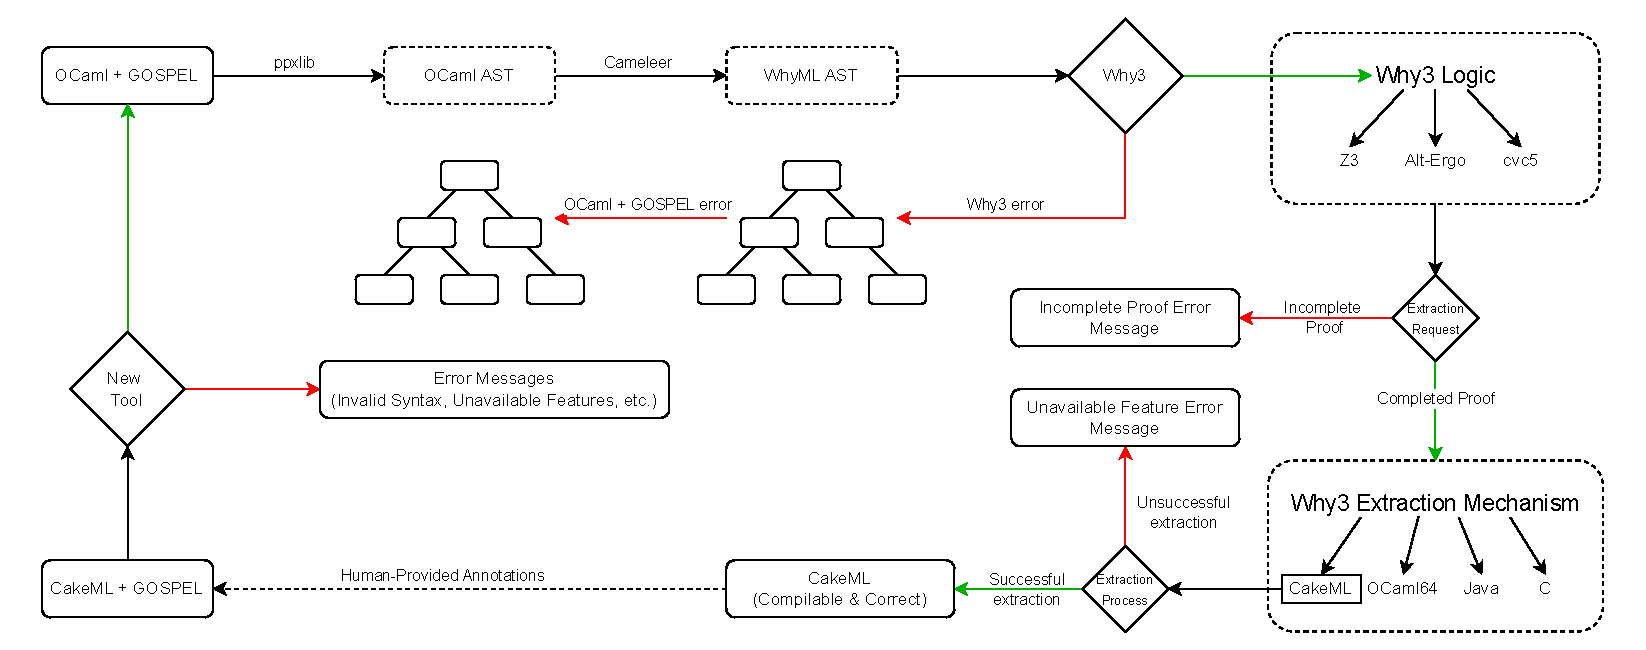
\includegraphics[width=\linewidth]{images/goal_pipeline.pdf}
    \caption{Goal pipeline}
    \label{fig:GoalPipeline}
\end{figure}

The pipeline in the previous figure \ref{fig:GoalPipeline} shows the two different approaches for deductive verification, extraction-based verification
and translation-based verification. These two approaches for deductive verification can be put through the same case studies, in order to take 
conclusions from their trust in the pipeline, ease of automation and the expressiveness in the specifications.

\section{Tool Modifications}

As shown in Figure \ref{fig:GoalPipeline}, which outlines the \cameleer pipeline, there is indirect support for \cml 
through \cameleer, but the current extraction mechanism uses the OCaml64 option. 
A small modification to the file \texttt{/bin/cli.ml} of \cameleer 's source code
\footnote{Original \cameleer code: \link{https://github.com/ocaml-gospel/cameleer/blob/master/bin/cli.ml}} 
\footnote{Modified \cameleer code: \link{https://github.com/TiagoMeirim/cameleer/blob/master/bin/cli.ml}}, 
allows the extraction to \cml. By changing the \inlinecode{execute\_extract} function to invoke 
\inlinecode{why3 extract -D cakeml \%s}, the tool can target \cml as a backend. With this adjustment, running 
\inlinecode{cameleer program.ml $--$extract} translates the original \ocaml plus \gospel code into code in the \cml language. 
This enables extraction from \ocaml directly into \cml, providing the basis for a verified compilation pipeline.

The alternative to this process is to obtain the code translated \whyml from running \cameleer with the flag \inlinecode{$--$debug} 
and then apply the mechanism of extraction of \whythree directly. Not only is this process more complex, but also the debug flag 
produces code that can not be opened by the \whythree platform because it contains proof goals directly in the code. This also implies
altering the code manually or to substantially modify the behaviour of the debug flag which is not intended.

\section{Case Studies}
\label{sec:Case_Studies}

For all the case studies below mentioned, the \ocaml + \gospel code was verified through \whythree automatic
provers before applying the extraction command to translate into \cml. This verification step is essential because the correctness 
guarantees of the final \cml code depend entirely on the validity of the specifications and their successful discharge by the 
provers. Without ensuring that the \whyml intermediate code satisfies the given specifications, the generated \cml code would 
no longer carry the desired formal guarantees, thereby breaking the intended end-to-end verification pipeline.

Since this step is intended only to demonstrate what already exists, the generated code may contain significant syntax errors 
and may not be compilable. These issues reflect limitations in the current extraction process and highlight the need for 
further refinement.

For presentation purposes we omitted parts of the original \ocaml + \gospel code in some of the case studies. The complete 
versions can be found in the appendix \ref{app:appendix}.

\subsection{Tail Recursive Factorial}

Initially an iterative version of the factorial function was also considered, however, since \cml does not support imperative loop 
constructs such as \inlinecode{for} or \inlinecode{while} we had to look for alternative versions of this example. Instead, we opted 
to study the tail recursive variant to simulate iteration, found in section \ref{subsec:CameleerExample}. The extracted code can be seen below:

\begin{cakeml}
fun fact_aux n c t = let val n1 = n in
  let val c1 = c in
  let val t1 = t in
  if c1 <= n1 then (fact_aux n1 (c1 + (1)) (t1 * c1))  else (t1)

fun fact n = let val n1 = n in fact_aux n1 (1) (1)
\end{cakeml}

The generated \cml code failed to compile due to differences in \inlinecode{let} expression syntax between \ocaml and \cml. In \cml, every 
\inlinecode{let} block must be explicitly closed with an \inlinecode{end} keyword, whereas in \ocaml, this is not required. It should
also be mentioned that the generated let-bindings generated are not necessary and only duplicate the variables in the arguments.

Initially we want to correct the let-binding termination as demonstrated in the following code:

\begin{cakeml}
fun fact_aux n c t = let val n1 = n in
  let val c1 = c in
  let val t1 = t in
  if c1 <= n1 then (fact_aux n1 (c1 + (1)) (t1 * c1))  else (t1)
  end end end

fun fact n = let val n1 = n in fact_aux n1 (1) (1) end
\end{cakeml}

However, our final goal is to eliminate as much unnecessary code as possible, in this case, the expendable let-bindings, while 
maintaining the desired behaviour:

\begin{cakeml}
fun fact_aux n c t = 
  if c <= n then (fact_aux n (c + (1)) (t * c))  else (t)

fun fact n = fact_aux n (1) (1)
\end{cakeml}

Both versions of this example are compilable and function correctly. This first example is simple and quite clearly demonstrates that
our pipeline can function if small changes are applied to the extraction mechanism.

\subsection{Exception recursive search}

One possible use of exceptions, although it may seem natural at first, can be to stop iteration early in \ocaml, for instance, in the 
context of linear search when the desired element is found, for more information regarding the implementation see section 
\ref{subsec:SearchCode}. Once again, since, for and while loops are not available in \cml to simulate iteration we use recursion 
with a counter:

\begin{gospell}
let rec search_aux a c n = (* ... *)
(*@
  r = search_aux a c n
  requires 0 <= c <= Array.length a
  requires forall k. 0 <= k < c -> a.(k) <> n
  raises Not_found -> forall k. 0 <= k < Array.length a -> a.(k) <> n
  ensures 0 <= r < Array.length a
  ensures a.(r) = n
  variant Array.length a - c
*)
\end{gospell}

Inside the \gospel specifications, we must guarantee that index \inlinecode{c} is between values of 0 and the length of the array 
\inlinecode{a}, which in turn gives us the assurance that the array is never accessed for values out of its range expect for the case 
where \inlinecode{c} is equal to the length in which case the function terminates without accessing the array. To further strengthen the
precondition above there is the need to state that all the values previously seen are not the desired value, otherwise the function
should have terminated earlier.

Since the exception \inlinecode{Not\_Found} was not handled this means that the function does not return a value in case it is raised,
therefore only when a value is found it terminates successfully. In that case, we need to express two ensure clauses, one that states 
the resulting index is a value between 0 and the length of the array a minus one and that the element of the array in the index returned 
is effectively the value searching for. As the index is increasing in each iteration, at some point it becomes equal to the length of the 
array, thereby proving termination and the variant clause.

The core function, \inlinecode{linear\_search}, delegates the search process to the auxiliary function that recursively traverses 
the array:

\begin{gospell}
let linear_search a n = search_aux a 0 n
(*@
  r = linear_search a n
  raises Not_found -> forall k. 0 <= k < Array.length a -> a.(k) <> n
  ensures 0 <= r < Array.length a
  ensures a.(r) = n
*)
\end{gospell}

Following the same train of thought, we must express the two possible outcomes. The first is when the \inlinecode{Not\_found} exception
is raised and the element was not found within the boundaries of the array. The second case is when the result is in fact an integer
inside the boundaries and the value inside the array in the index provided is the same value being searched.

This makes the function verifiable by \whythree before attempting extraction to \cml, ensuring that key correctness properties are 
formally validated. The extracted code is:

\begin{cakeml}
fun search_aux a c n = let val a1 = a in
  let val c1 = c in
  let val n1 = n in
  let exception Break of (int) in
  ((if c1 = (a1.length) then (raise Not_found) 
    else (if (get a1 c1) = n1 then (raise (Break n1)) 
          else (search_aux a1 (c1 + (1)) n1)))
  handle   Break i => i)

fun linear_search a n =
  let val a1 = a in let val n1 = n in search_aux a1 (0) n1
\end{cakeml}

The generated \cml code fails to compile due to several incompatibilities between \ocaml and \cml that must be addressed 
to ensure a successful and semantically correct extraction. One of the primary issues concerns exception handling, as \cml 
requires all exceptions to be declared globally, outside the scope of functions, whereas the extracted code attempts to define 
the exception Break locally within a function using let-bound exception, a construct that is not valid in \cml. This syntactic 
difference results in a compilation error and reflects a broader incompatibility in exception scoping between the two languages.

Additionally, array operations in \cml differ substantially from those in \ocaml. While \ocaml allows for concise access through 
expressions like \inlinecode{a.(i)} while \cml demands the usage of a function from the array library \inlinecode{Array.sub a i}. 
The generated code fails in this aspect by using invalid expressions such as \inlinecode{a1.length} and \inlinecode{get a1 c1}, 
neither are supported by the \cml standard library nor array library. This divergence in the array library further contributes 
to the failure of the generated code to compile.

Moreover, the problems with let-bindings discussed earlier also contribute to another critical issue. These problems collectively 
illustrate the importance of a properly configured and semantically aware translation mechanism. The corrected code is presented below:

\begin{cakeml}

exception Not_found
exception Break int

fun search_aux a c n =
  ((if c = (Array.length a) then (raise Not_found) 
    else (if (Array.sub  a c) = n then (raise (Break n)) 
          else (search_aux a (c + (1)) n)))
  handle Break i => i)

fun linear_search a n = search_aux a (0) n

\end{cakeml}

With this example we wanted to showcase how the extraction mechanism translates array definitions, access and other operations 
as well as handling exceptions.

\subsection{Count Even For A List}

Since operations for arrays have already been explored in the previous case study, we also want to explore if the same happens with
operations for lists. We also utilize the mod operator from the standard library, when trying to count every even number 
inside a given list:

\begin{gospell}
let count_even l =
  let l1 = List.filter (fun x -> x > 0 && x mod 2 = 0) l in
  let l2 = List.rev l1 in
  (List.length l2, l2)
(*@ (s, r) = count_even l
    ensures s = List.length r
    ensures forall x: int. List.mem x r -> x > 0 && mod x 2 = 0 
    ensures forall x: int. List.mem x r -> List.mem x l
    ensures forall x: int. not List.mem x l -> not List.mem x r *)
\end{gospell}

The function \inlinecode{count\_even} receives as the sole argument the list to be searched. The following code for the \inlinecode{l1}
is to apply a filter for the original list \inlinecode{l}, where inside the filter we only want values that are positive and even.
Theoretically, the operation is already done, but for research purposes we added more operations to see how the translation would undergo
for different operations, those where the inversion of the list and the length of a list.

The specification passes through ensuring some crucial information. As the function is organized, it returns a tuple with both the 
corresponding length of the list created and the list created, so, we start by comparing the first element of the tuple, which should 
be the length of the reversed and filtered list, and therefore equal to the length of the second argument, the same list. Then there is 
a need to guarantee all the values inside the created list are effectively positive and even. Additionally, every element belonging 
inside the list created is also inside the original list and every value that is not inside the original list is not inside the created 
list. For simplicity, we do not guarantee that the number of occurrences for each number that belong to the resulting list is also 
the same as the original list. This condition would guarantee of this function however its proof would be complex to display here.

The extracted code can be seen below:

\begin{cakeml}
fun count_even l =
  let val l1 = l in
  let val l11 = filter (fn x => (x > (0)) andalso ((mod x (2)) = (0))) l1 in
  let val l2 = rev l11 in (List.length l2, l2)
\end{cakeml}

The list operations are not correctly declared, it seems only the length operation is written with the correct syntax. The mod operator
is used as if it is a function from the standard library, however in \cml it is part of the \inlinecode{Int} library. The duplicate 
let-bindings were also generated for every argument.

Correcting the code, becomes the block below:

\begin{cakeml}
fun count_even l =
  let val l1 = List.filter (fn x => (x > (0)) andalso ((Int.mod x (2)) = (0))) l in
  let val l2 = List.rev l1 in (List.length l2, l2) end end
\end{cakeml}

Using the correct syntax for calling every list operation and integer operation while deleting all the unnecessary let-bindings makes the
code compilable and correct.

% \subsection{High-order}

% In the documentation for \cml it was not possible to find any mention of higher-order functions. As such, we devised an example that
% combines higher order with pattern matching and lists. The function in this example multiplies all the values of a list by a certain
% integer:

% \begin{gospell}
% let rec mult_list l n =
%     match l with
%     | [] -> []
%     | h :: t -> n * h :: mult_list t n
% (*@ r = mult_list l n
%         ensures r = map (fun x -> x * n) l
%         variant l *)
% \end{gospell}

% This recursive function \inlinecode{mult\_list} receives as arguments a list and a value that is used to multiply on each of the
% lists values, one by one, using the pattern matching and a recursive call on the tail.

% The original list has its values extracted one by one until the list is empty, signalling the function termination, which in turn is 
% represented by the variant clause. The function \inlinecode{map} is classical example of function programming that applies another 
% function to all elements of a list. One can observe that the \inlinecode{mult\_list} function is a particular case of the \inlinecode{map} 
% function, where the function is the multiplication by a given integer n and is expressed by an anonymous function. 

% The logical implementation of the \inlinecode{map} function is presented below:

% \begin{gospell}
% (*@ function rec map (f: int -> int) (l: int list) : int list = 
%         match l with
%         | [] -> []
%         | h::t -> (f h) :: map f t *)
% (*@ variant l
%         ensures List.length result = List.length l *)
% \end{gospell}

% The logical function \inlinecode{map} represents the application of a certain function to the values of the list provided. For the same
% reason, the variant clause is represented by the list, since the termination for this logical function is also determined by when the
% list is empty. The is also the need to ensure that the length of the list resulting from applying the function to the original list
% is the same since the number of values do not change with this transformation.

% The corresponding generated code is:

% \begin{cakeml}
% fun mult_list l n = let val l1 = l in
%     let val n1 = n in
%     (case l1 of
%         [] => []
%     | h :: t => (n1 * h) :: (mult_list t n1))
% \end{cakeml}

% We can observe that pattern matching and basic list handling seems to be working well after the translation, however the extraction 
% still generates clones of the arguments, the code can not be compilable. 

% By solving the issues found, we tested the code and effectively, high-order functions are allowed by the compiler in \cml. The corrected 
% code is displayed below:

% \begin{cakeml}
% fun mult_list l n =
%     (case l of
%         [] => []
%     | h :: t => (n * h) :: (mult_list t n))
% \end{cakeml}

% Since the issue continues to stem from the let-bindings, the solution to add the termination token or eliminating the unnecessary 
% let-bindings still seems to solve the problem at hand.

\subsection{Depth-search tree}

User defined data types, such as trees, are very important for real world examples in functional programming, since traversing them
can easily be achieved recursively. For the tree data structure definition can be found in section \ref{subsec:ADT}. The recursive 
depth-first search algorithm for trees can be implemented as:

\begin{gospell}
let rec depth_search t n = 
  match t with
  | Leaf -> false
  | Node (l,x,r) -> x = n || depth_search l n || depth_search r n
(*@
  r = depth_search t n
  variant t
  ensures List.mem n (to_list t) <-> r
*)
\end{gospell}

The following recursive function \inlinecode{depth\_search} shows how a tree is traversed through its depth firstly when trying to find
a node that has the same value as the value given in the arguments.

Since the algorithm searches the subtree to the left and subtree to the right it is known that each of those trees is smaller than their
parent. In the worst case, where the element is not found in the tree, we know that recursion terminates with the leaves, so the variant 
clause is the tree that was searched. One way to guarantee the result is correct is to transform the tree into a list and checking if
the desired element is found in the resulting list with the \inlinecode{List.mem} operation.

To transform the tree into a list we formed an auxiliary logical function:

\begin{gospell}
(*@ function rec to_list (t: 'a tree) : 'a list = 
  match t with
  | Leaf -> []
  | Node l x r -> x :: to_list l @ to_list r
*)
(*@
  variant t
*)
\end{gospell}

The recursive function \inlinecode{to\_list} transforms a tree firstly from the own element of the root, following the left side and 
ending with the right side. Since, for this example, we are only concerned with the inclusion of an element in the list, the order 
in which it is constructed doesn't have effect on the outcome of the solution, our decision was arbitrary.

Similarly to the function \inlinecode{depth\_search}, the termination can be proven by the tree itself.

The generated \cml code was:

\begin{cakeml}
'a datatype tree = Leaf | Node of 'a tree * 'a * 'a tree

fun depth_search t n = let val t1 = t in
  let val n1 = n in
  (case t1 of
    Leaf => false
  | Node l x r =>
    (x = n1) orelse ((depth_search l n1) orelse (depth_search r n1)))
\end{cakeml}

The definition of the tree data type is incorrect for three reasons. Number one the ordering of the syntax for the left side declaration 
of a data type starts with the token \inlinecode{datatype} and only after the generic type \inlinecode{'a}. The second reason is the
unnecessary token \inlinecode{of} that is not used when declaring a tuple in \cml syntax. Thirdly, the tokens \inlinecode{*} are also
unnecessary when declaring tuples. Finally, the let-bindings displayed the same errors as previous examples.

The corrected code below:

\begin{cakeml}
datatype 'a tree = Leaf | Node ('a tree) 'a ('a tree)

fun depth_search t n =
  (case t of
    Leaf => False
  | Node l x r =>
    (x = n) orelse ((depth_search l n) orelse (depth_search r n)))
\end{cakeml}

Correcting the order and removing the unnecessary tokens in data type definition, achieves a more robust extraction mechanism that 
produces compilable \cml code.

\subsection{Tree Comparison}

With this example we only want to understand if the module system is working as intended in \cml. The module system in \cml is very 
limited since it does not support signatures and functors. In section \ref{subsec:ModuleSystem} we present a simple tree module in \ocaml that 
contains the comparison between trees. Below it is shown the necessary \gospel annotations:

\begin{gospell}
module Tree = struct
  type 'a tree = (* ... *)

  let rec cmp t1 t2 = (* ... *)
  (*@
  r = cmp t1 t2
  variant t1
  ensures r <-> t1 = t2
  *)
end
\end{gospell}

Logically, the result should be equal to comparing \inlinecode{t1} and \inlinecode{t2} and the variant clause could be either one of 
the trees since it only matters when the result is correct therefore the trees have the same structure, and in each recursive call we
are considering fewer elements until, eventually, there are no more elements.

Generated code to \cml was:

\begin{cakeml}
'a datatype tree = Leaf | Node of 'a tree * 'a * 'a tree

fun cmp t1 t2 = let val t11 = t1 in
  let val t21 = t2 in
  (case (t11, t21) of
    (Leaf, Leaf) => true
  | (Leaf, _) => false
  | (_, Leaf) => false
  | (Node l1 x1 r1, Node l2 x2 r2) =>
    (cmp l1 l2) andalso ((x1 = x2) andalso (cmp r1 r2)))
\end{cakeml}

Once more, the data types and let-bindings expressions failed to extract correctly, but more notably the module is not present.
The corrected version is demonstrated below:

\begin{cakeml}
structure Tree = struct
  datatype 'a tree = Leaf | Node ('a tree) 'a ('a tree)

  fun cmp t1 t2 =
  (case (t1, t2) of
    (Leaf, Leaf) => True
  | (Leaf, _) => False
  | (_, Leaf) => False
  | (Node l1 x1 r1, Node l2 x2 r2) =>
      (cmp l1 l2) andalso ((x1 = x2) andalso (cmp r1 r2)))
end
\end{cakeml}

For the same problems, the same solutions were implemented, While modules are not explicitly shown
in \cml's documentation, by having a look at SML's module syntax, it was possible to reach the 
\inlinecode{structure Tree = struct ... end} construct, which was not presented in the translated code.

\subsection{References}

To demonstrate support for references, a program was implemented to perform Euclidean division, also known as division with remainder. 
This operation involves dividing one non-negative integer by another positive integer, resulting in two values: a positive integer 
quotient and a non-negative remainder that is strictly less than the absolute value of the divisor. This program is demonstrated 
in the section \ref{subsec:SideEffects} and its specification is presented below:

\begin{gospell}
let rec eudiv_aux (x: int) (y: int) (r: int ref) (q: int ref) = (* ... *)
(*@ res = eudiv_aux x y r q
    requires x >= 0
    requires y > 0
    requires 0 <= !r <= x
    requires x = y * !q + !r
    variant !r - y
    ensures x = y * !q + !r
    ensures 0 <= !r <= x
    ensures 0 <= !r < y *)
\end{gospell}

To specify this function, we used \gospel annotations to define pre-conditions and post-conditions that ensure the correctness of 
the Euclidean division. The pre-conditions enforce that the dividend must be a non-negative integer, the divisor must be strictly 
positive, and the remainder (held in a reference) must initially lie between 0 and the dividend. Additionally, we specify that the 
dividend is equal to the product of the divisor and quotient plus the remainder at each recursive call. For the post-conditions, we 
ensure that this equation is preserved after execution. Furthermore, the remainder must always remain non-negative and strictly less 
than the divisor, which aligns with the definition of Euclidean division. In every iteration, we subtract \inlinecode{y} from the
remainder \inlinecode{\!r} so a natural way to guarantee termination is to use this exact expression as a variant condition.

\begin{gospell}
let euclidean_div x y = (* ... *)
(*@ (q, r) = euclidean_div x y
    requires x >= 0
    requires y > 0
    ensures x = y * q + r
    ensures 0 <= r < y *)
\end{gospell}

The \gospel specifications require the dividend to be a non-negative integer and the divisor to be strictly positive. The function 
ensures that the dividend always equals the product of the divisor and the quotient plus the remainder. Additionally, it guarantees 
that the remainder remains non-negative and strictly less than the divisor, as defined by the Euclidean division properties.

The translated code to \cml is represented below:

\begin{cakeml}
fun eudiv_aux x y r q = let val x1 = x in
  let val y1 = y in
  let val r1 = r in
  let val q1 = q in
  if (!r1) >= y1
  then ((r1 := ((!r1) - y1); q1 := ((!q1) + (1)); eudiv_aux x1 y1 r1 q1))

fun euclidean_div x y =
  let val x1 = x in
  let val y1 = y in
  let val r = ref x1 in
  let val q = ref (0) in (eudiv_aux x1 y1 r q; (!q, !r))
\end{cakeml}

The operations concerning references, creation, assignment and access, all seem to be well translated syntactically, the problem with
let-bindings is recurring, however a new issue arises as the \inlinecode{else} branch with a single unit value was not generated for the 
function \inlinecode{eudiv\_aux}.

The following code for \cml is the corrected version:

\begin{cakeml}
fun eudiv_aux x y r q =
  if (!r) >= y
  then ((r := ((!r) - y); q := ((!q) + (1)); eudiv_aux x y r q))
  else ()

fun euclidean_div x y =
  let val r = Ref x in
  let val q = Ref (0) in (eudiv_aux x y r q; (!q, !r)) 
    end end
\end{cakeml}

Removing the unnecessary let-bindings and correctly handling of the \inlinecode{else} branch, which was absent, the functions became 
both syntactically correct and successfully compilable.

\section{Analyses For The Case Studies}

During our studies we found various issues, such as exception scoping, array operation semantics, and let-binding syntax, the extracted 
code remains invalid and cannot serve as a verified executable target. Therefore, improving the extraction pipeline from \ocaml and 
\gospel to \cml necessitates careful handling of these language specific constructs to ensure that the resulting code is not only 
syntactically correct but also preserves the behaviour of the original verified source.
